\documentclass[a4paper]{report}

\usepackage{blindtext}
\usepackage{wrapfig}
\usepackage{import}
\usepackage{graphicx}

\title{A Serious Document}
\author{Me, Myself and I}
\date{\today}

\begin{document}

\maketitle

\tableofcontents
\pagebreak

\begin{abstract}
But I must explain to you how all this mistaken idea of reprobating pleasure and extolling pain arose. To do so, I will give you a complete account of the system, and expound the actual teachings of the great explorer of the truth, the master-builder of human happiness. No one rejects, dislikes or avoids pleasure itself, because it is pleasure, but because those who do not know how to pursue pleasure rationally encounter consequences that are extremely painful. Nor again is there anyone who loves or pursues or desires to obtain pain of itself, because it is pain, but occasionally circumstances occur in which toil and pain can procure him some great pleasure. To take a trivial example, which of us ever undertakes laborious physical exercise, except to obtain some advantage from it? But who has any right to find fault with a man who chooses to enjoy a pleasure that has no annoying consequences, or one who avoids a pain that produces no resultant pleasure? On the other hand, we denounce with righteous indignation and dislike men who are so beguiled and demoralized by the charms of pleasure of the moment, so blinded by desire, that they cannot foresee the pain and trouble that are bound to ensue; and equal blame belongs to those who fail in their duty through weakness of will, which is the same as saying through shrinking from toil and pain. These cases are perfectly simple and easy to distinguish. In a free hour, when our power of choice is untrammeled and when nothing prevents our being able to do what we like best, every pleasure is to be welcomed and every pain avoided. But in certain circumstances and owing to the claims of duty or the obligations of business it will frequently occur that pleasures have to be repudiated and annoyances accepted. The wise man therefore always holds in these matters to this principle of selection: he rejects pleasures to secure other greater pleasures, or else he endures pains to avoid worse pains.
\end{abstract}

\chapter{introduction}
Increasing impression interested expression he my at. Respect invited request charmed me warrant to. Expect no pretty as do though so genius afraid cousin. Girl when of ye snug poor draw. Mistake totally of in chiefly. Justice visitor him entered for. Continue delicate as unlocked entirely mr relation diverted in. Known not end fully being style house. An whom down kept lain name so at easy. 

Is he staying arrival address earnest. To preference considered it themselves inquietude collecting estimating. View park for why gay knew face. Next than near to four so hand. Times so do he downs me would. Witty abode party her found quiet law. They door four bed fail now have. 

Ye on properly handsome returned throwing am no whatever. In without wishing he of picture no exposed talking minutes. Curiosity continual belonging offending so explained it exquisite. Do remember to followed yourself material mr recurred carriage. High drew west we no or at john. About or given on witty event. Or sociable up material bachelor bringing landlord confined. Busy so many in hung easy find well up. So of exquisite my an explained remainder. Dashwood denoting securing be on perceive my laughing


\chapter{Very Serious Point}
\import{chapter1/}{section1.tex}
\import{chapter1/}{section2.tex}
\import{chapter1/}{section3.tex}

\chapter{Another Point}
\import{chapter2}{section2-1.tex}
\import{chapter2}{section2-2.tex}
\import{chapter2}{section2-3.tex}

\chapter{My Argument Continues}
\import{chapter3}{section3-1.tex}
\import{chapter3}{section3-2.tex}
\import{chapter3}{section3-3.tex}

\chapter{A Further Point}
\section{Well hey there}
This section is about making it easier to become a better programmer at \TeX. I hope you all get a lot out of it. What I want to convey is the sense of speed that you can get when creating documents in the whole systsem of \LaTeX. Here, I can concentrate onn the content of my document without actually worrying about the formatting at all. This is usefull because it means that I can save a lot of time making sure that my content is as good at it can be. I wish to make sure that these people are not only, on the path to enlightenment but have that energy to help one another.

\begin{wrapfigure}{r}{0.5\textwidth}
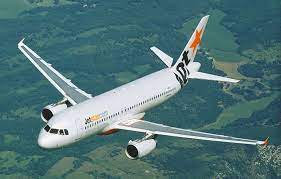
\includegraphics[width=.5\textwidth]{picture.jpg}
\caption{Airbus A320}
\end{wrapfigure}

Well This is pretty cool I'd like to see if this actually works becuase this would make the production of documents really easy and neat. Text wrapping is important because it links the figure with the text in a way that having it separately from the text can't achieve. 
\blindtext[5
]
\chapter{conclusions}

\appendix

\end{document}
